%%% TITLE AND AUTHORS %%%%%%%%%%%%%%%%%%%%%%%%%%%%%%%%%%%%%%%%%%%%%%%%%%%%%%%%%
\title[Digital Footprints \& Micro-targeting]{
    Digital Footprints and Micro-targeting
}
\author[]{Szymon Talaga and Mikołaj Biesaga} % Your name
\institute[ISS UW]{
    The Robert Zajonc Institute for Social Studies \\ University of Warsaw \\
    \medskip
    \textcolor{blue}{\href{mailto:stalaga@uw.edu.pl}{stalaga@uw.edu.pl}} \\
    \textcolor{blue}{\href{mailto:m.biesaga@uw.edu.pl}{m.biesaga@uw.edu.pl}}
}
\date{9 October 2019} % Date, can be changed to a custom date

%%% SLIDES %%%%%%%%%%%%%%%%%%%%%%%%%%%%%%%%%%%%%%%%%%%%%%%%%%%%%%%%%%%%%%%%%%%%
\frame{\titlepage}

\section[Fun Facts]{Fun Facts}

\begin{frame}
    \frametitle{Access to Internet}
    According to Measuring the Information Society Report 2018 51.2\% $\approx$ 3.9 billion people were using Internet in 2018:
        \begin{itemize}
            \item 80\% in Developed countries
            \item 45\% in Developing countries
            \item 20\% in 47 least-developed countries
        \end{itemize}
    According to GUS 2019 in Poland access to Internet had:
        \begin{itemize}
            \item 84\% of Households
            \item 99.7\% of Financial Sector Enterprises
            \item 95\% of Non-Financial Sector Enterprises
        \end{itemize}
\end{frame}

\begin{frame}
    \frametitle{Mobile Network}
    \only<+>{
        \begin{figure}
            \caption{Mobile cellular subscription (per 100 people)}
            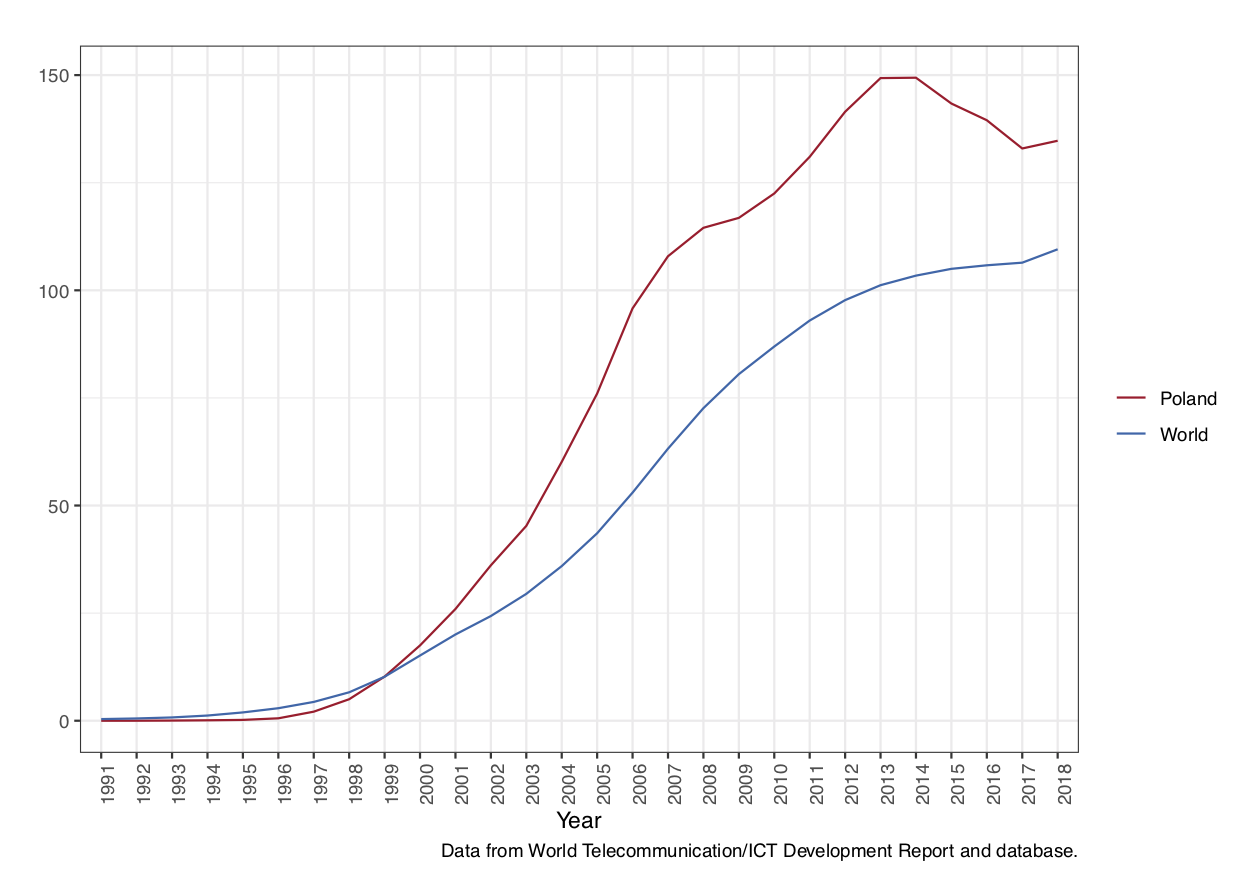
\includegraphics[width = \textwidth]{png/mobile_phones.png}
        \end{figure}
    }
    \only<+>{
        \begin{figure}
            \caption{Mobile phone internet user penetration worldwide from 2014-2019}
            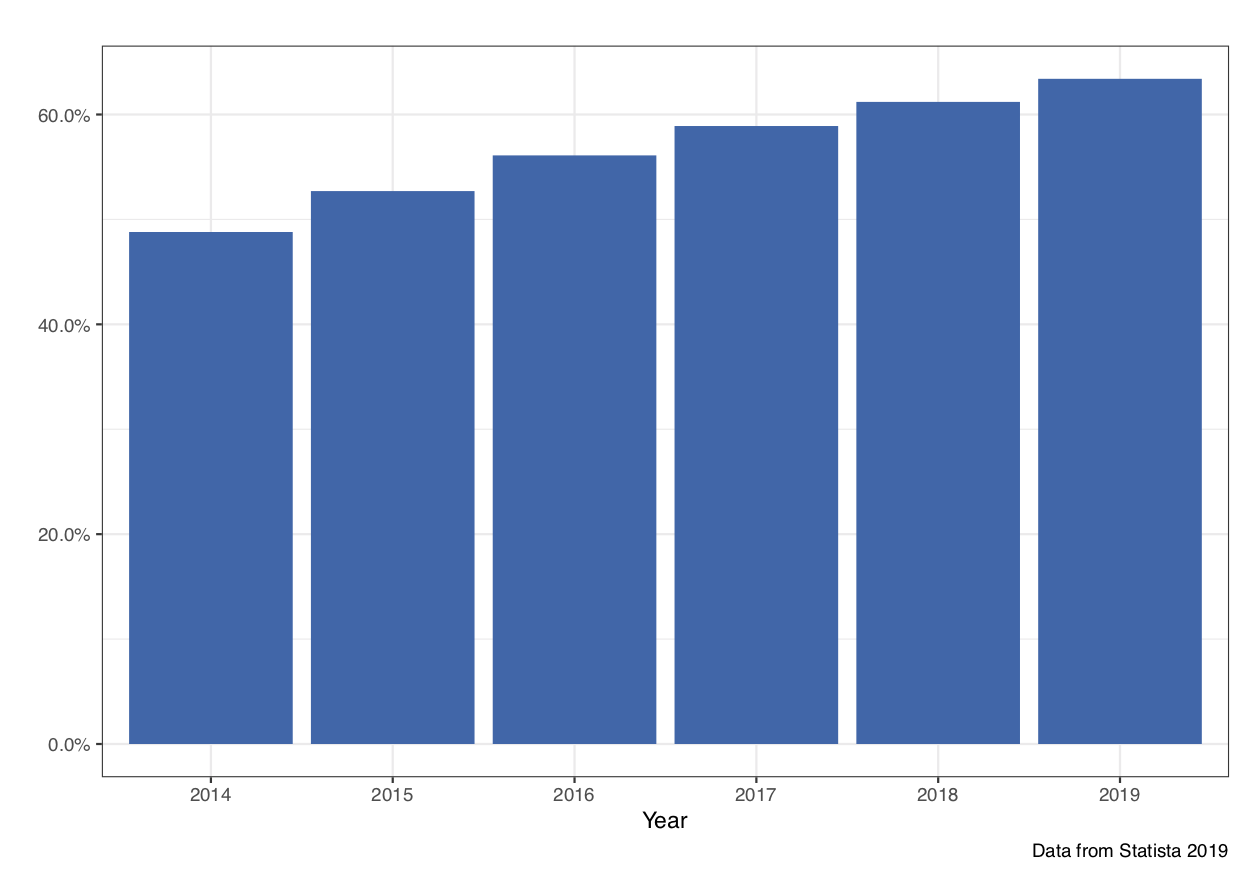
\includegraphics[width = \textwidth]{png/mobile_internet.png}
        \end{figure}
    }
\end{frame}

\begin{frame}
    \frametitle{Social Media}
    \captionsetup{labelformat=empty,labelsep=none}
    \only<+>{
        \begin{columns}[t]
            \begin{column}{.2\textwidth}
                \resizebox{\textwidth}{!}{
                
\includegraphics{png/facebook.png}}
                \resizebox{\textwidth}{!}{
                
\includegraphics{png/reddit.png}}
            \end{column}
            \begin{column}{.2\textwidth}
                \resizebox{\textwidth}{!}{
                
\includegraphics{png/instagram.png}}
                \resizebox{\textwidth}{!}{
                
\includegraphics{png/whatsapp.png}}
            \end{column}
            \begin{column}{.2\textwidth}
                \resizebox{\textwidth}{!}{
                
\includegraphics{png/twitter.png}}
                \resizebox{\textwidth}{!}{
                
\includegraphics{png/linkedin.png}}
            \end{column}
            \begin{column}{.2\textwidth}
                \resizebox{\textwidth}{!}{
                
\includegraphics{png/youtube.png}}
                \resizebox{\textwidth}{!}{
                
\includegraphics{png/pinterest.png}}
            \end{column}
        \end{columns}
    }
    \only<+>{
        \begin{table}
            \begin{tabular}{l | c }
                Servie & Users \\
                \hline \hline
                Facebook & 2.3 billion users \\
                YouTube & 1.9 bilion users \\
                Whatsapp & 1.6 bilion users \\
                Instagram & 1 billion \\
                Lindekin & 610 milion users\\
                Reddit & 542 milion users\\
                Twitter & 321 milion users \\
                Pinterest & 265 milion users\\
            \end{tabular}
            \caption{Data From Wikipedia}
        \end{table}
    }
    \only<+>{
        According to \href{https://www.brandwatch.com/blog/amazing-social-media-statistics-and-facts/}{\textcolor{blue}{brandwatch.com}}:
        \begin{itemize}
            \item the Internet has 4.4 billion users
            \item there are 3.499 billion active social media users
            \item the average time spent on social media is 142 minutes
            \item 74 billion dollars were spent on social media advertising in 2018
        \end{itemize}
    }
\end{frame}

\section[Digital Footprints]{Digital Footprints}
\begin{frame}
    \frametitle{Digital Footprints}
    \captionsetup{labelformat=empty,labelsep=none}
    \only<0>{
        \resizebox{\textwidth}{!}{
        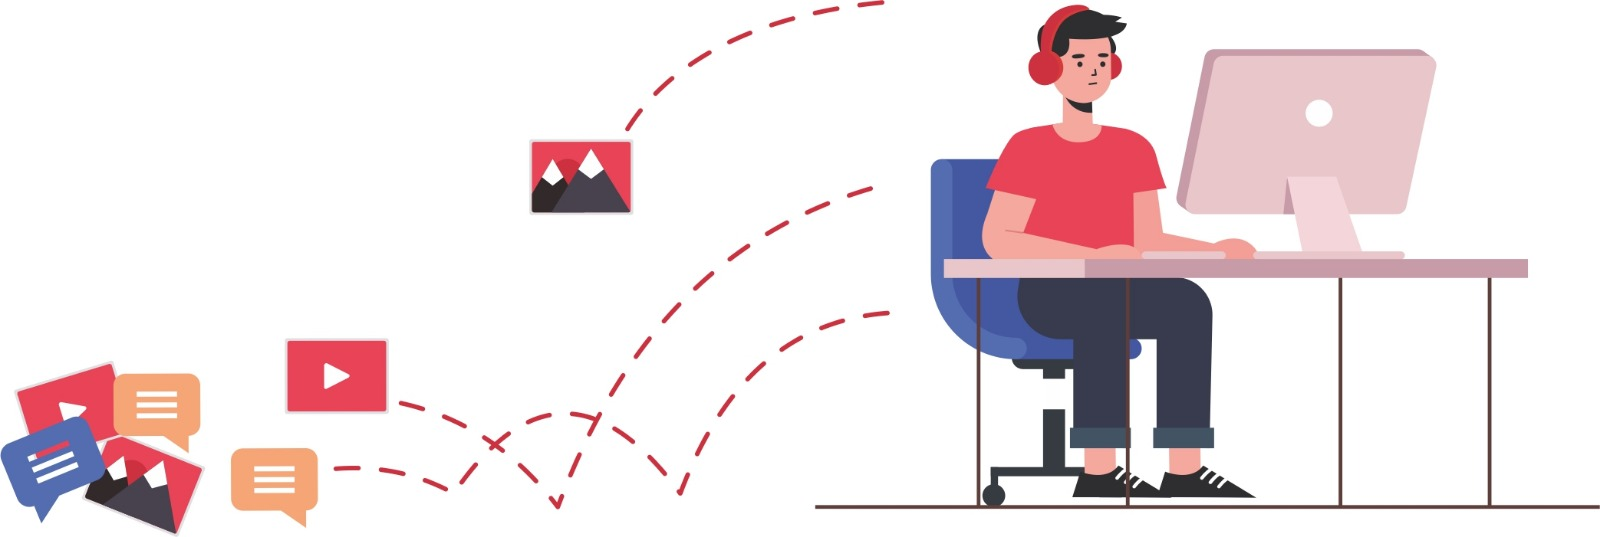
\includegraphics{png/digital_footprint.jpeg}}
    }
    \only<+>{
        \begin{figure}
            
\includegraphics[width = \textwidth]{png/ISOC-Dark-RGB_Logo_400px.png}
            \caption{ \href{https://www.youtube.com/watch?v=Ro_LlRg8rGg}{\textcolor{blue}{YouTube clip}}}
        \end{figure}
        }
    \only<+>{
        \begin{definition}
            \emph{Digital Footprint} (or digital shadow) is a unique traceable set of actions, contributions or communications manifested on the Internet or digital devices. In general, there are two types of digital footprints: passive and active.
        \end{definition}
        }
    \only<+>{
        \begin{definition}
            \emph{Passive Digital Footprint} is a trail of data you create unintentionally, i.e. when you visit the webserver may log your IP address, which identifies your Internet service provider and your approximate location.
        \end{definition}
    }
    \only<+>{
        \begin{definition}
            \emph{Active Digital Footprint} includes data that you intentionally submit online. Sending an email contributes to your active digital footprint since you expect the data to be seen and/or saved by another person.
        \end{definition}
    }
\end{frame}

\section[Micro-targeting]{Micro-targeting}
\begin{frame}
    \frametitle{Micro-targeting}
    \only<+>{
        \begin{definition}
            In general terms, \emph{micro-targeting} is sending a message to a highly specific portion of an audience based on particular information.
        \end{definition}
    }
    \only<+>{
        \begin{figure}
            \centering
            
\includegraphics[scale = .25]{png/targetlogo-6.jpeg}
            \caption{from \href{https://corporate.target.com/article/2014/04/bullseye-love-history-of-target-logo}{\textcolor{blue}{www.corporate.target.com}}}
        \end{figure}
    }
    \only<+>{
        \resizebox{\textwidth}{!}{
        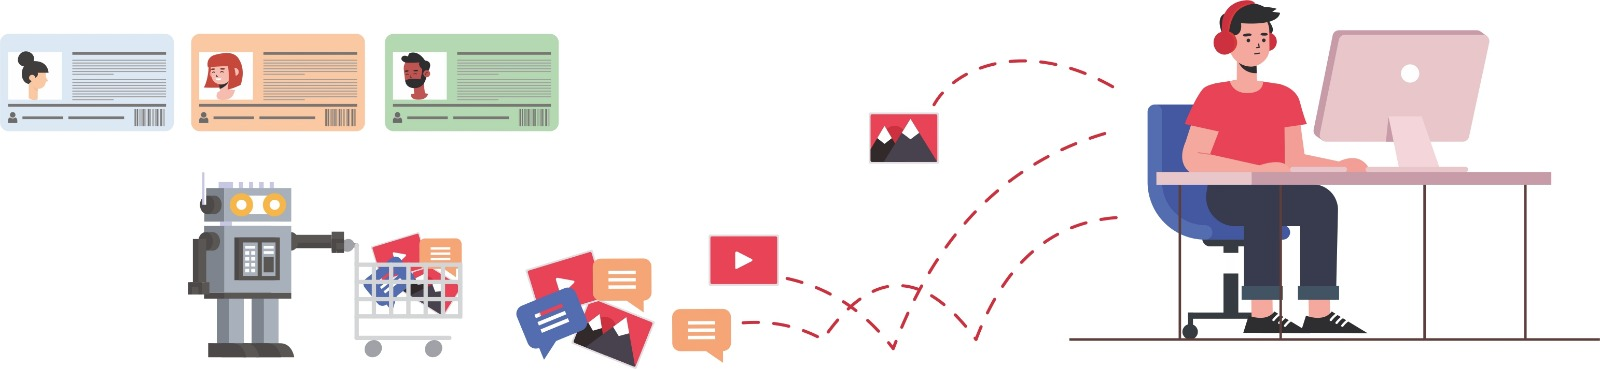
\includegraphics{png/microtargeting.jpeg}}
    }

\end{frame}

\subsection[Facebook Studies]{Psychological Targeting}
\begin{frame}
    \frametitle{Psychological Targeting}
    \only<1,4>{
        \begin{itemize}
            \item 2007 David Stillwell creates \href{https://sites.google.com/michalkosinski.com/mypersonality}{\textcolor{blue}{myPersonality}} Facebook App to share a personality questionnaire
            \item by 2012 6 million people completed personality questionnaire
            \item 40\% of participants gave the informed consent to share their Facebook data
            \item Private traits and attributes are predictable from digital records of human behavior (\cite{Kosinski2013})
            \item<4> Psychological targeting as an effective approach to digital mass persuasion (\cite{Matz12714}; \cite{EcklesE5254}; \cite{SharpE7890})
        \end{itemize}
    }
    \only<2>{
        \begin{figure}
            \centering
            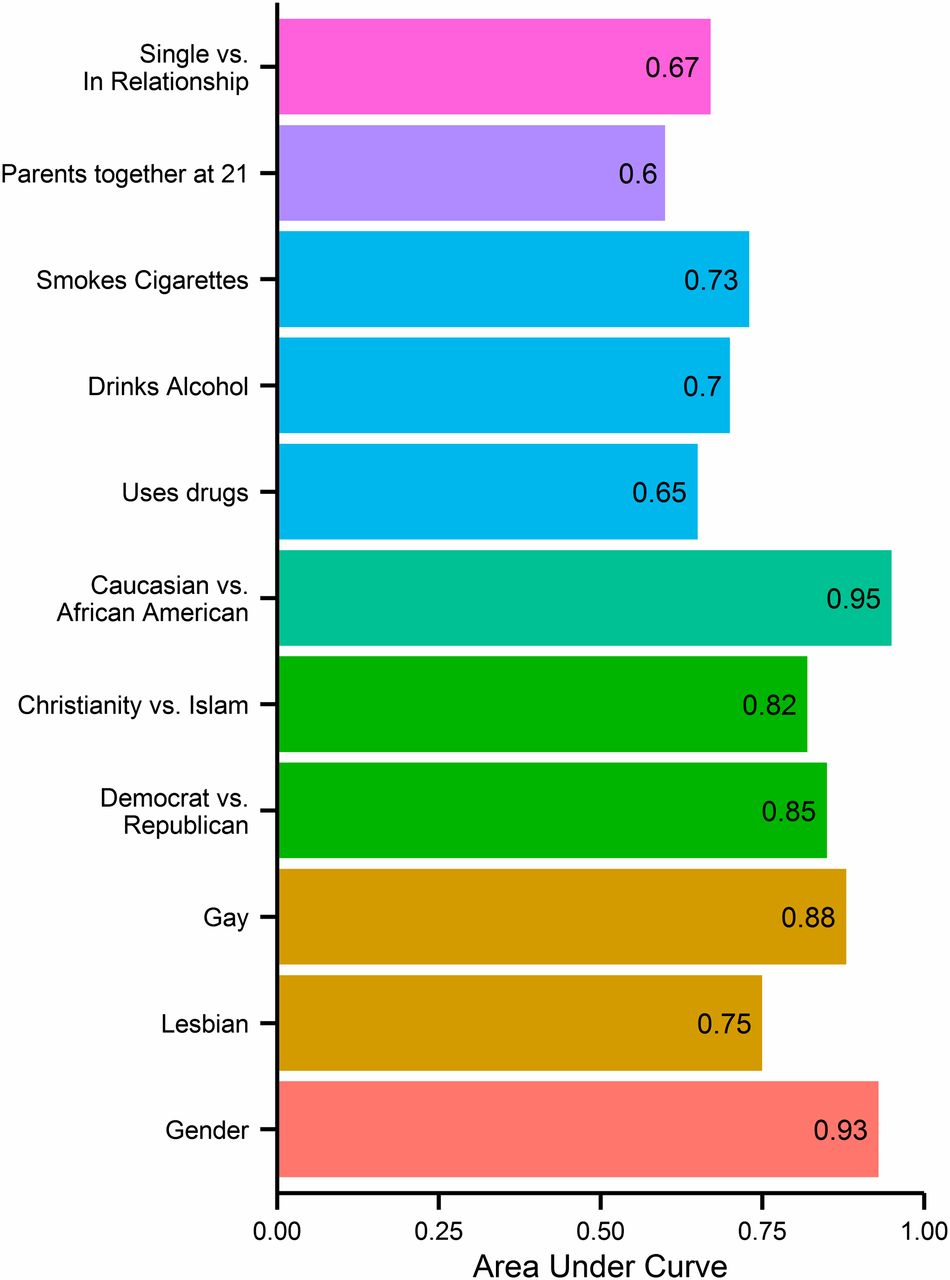
\includegraphics[scale = .7]{png/Kosinski_S1.jpg}
            \caption{\cite{Kosinski2013}}
        \end{figure}
    }
    \only<3>{
        \begin{figure}
            \centering
            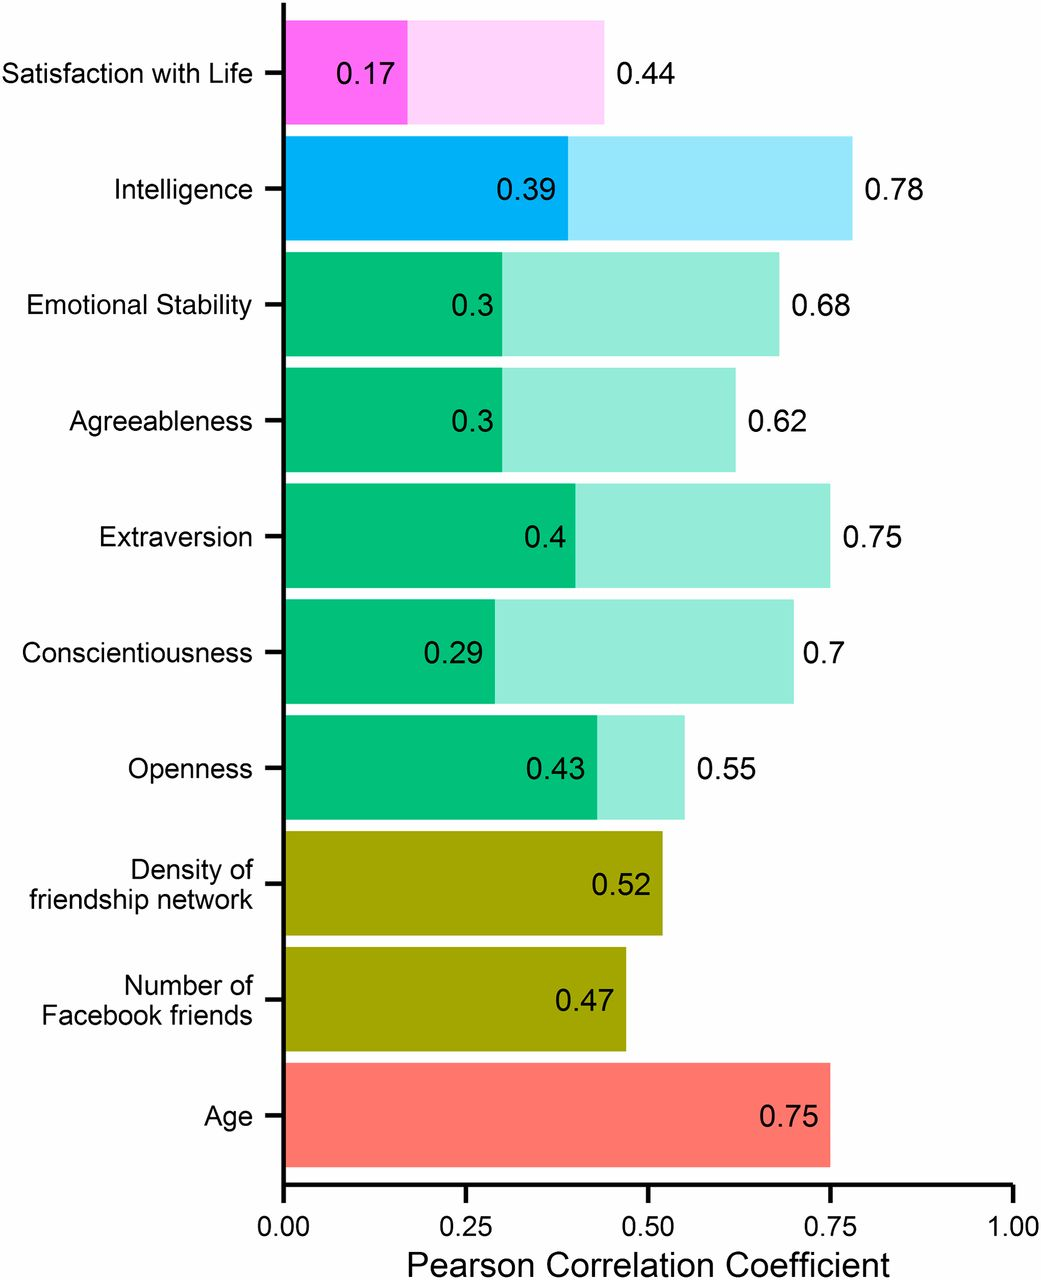
\includegraphics[scale  =.7]{png/Kosinski2_S1.jpg}
            \caption{\cite{Kosinski2013}}
        \end{figure}
    }
    \only<5>{
        \begin{figure}
            \centering
            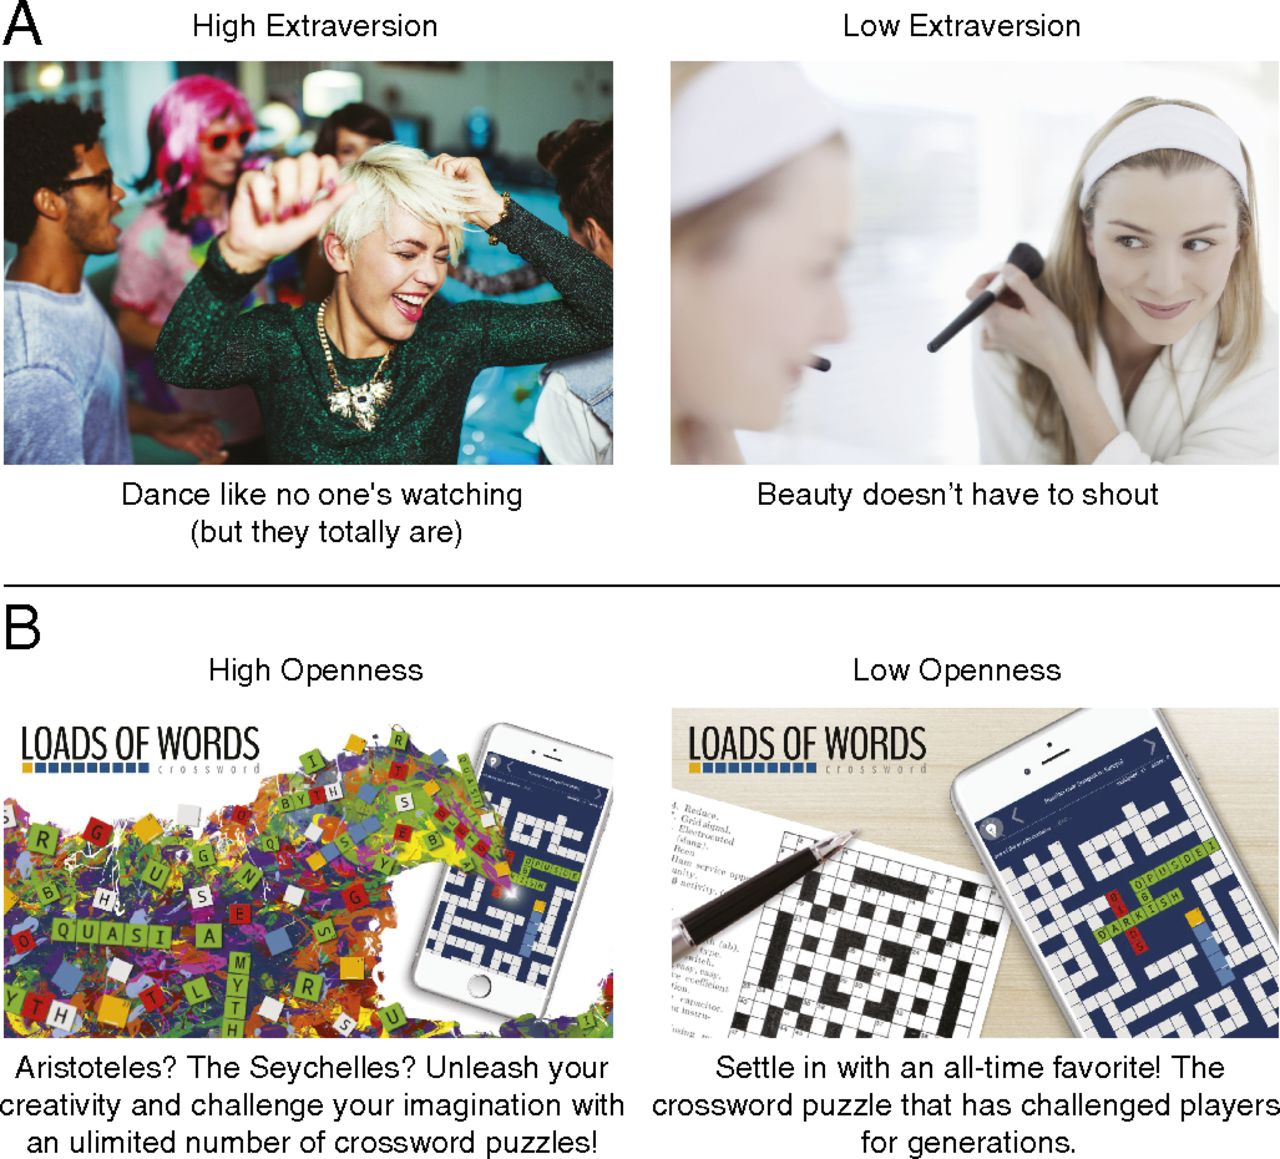
\includegraphics[scale = .7]{png/Kosinski_S2.jpg}
            \caption{\cite{Matz12714}}
        \end{figure}
    }
    \only<6>{
        \begin{figure}
            \centering
            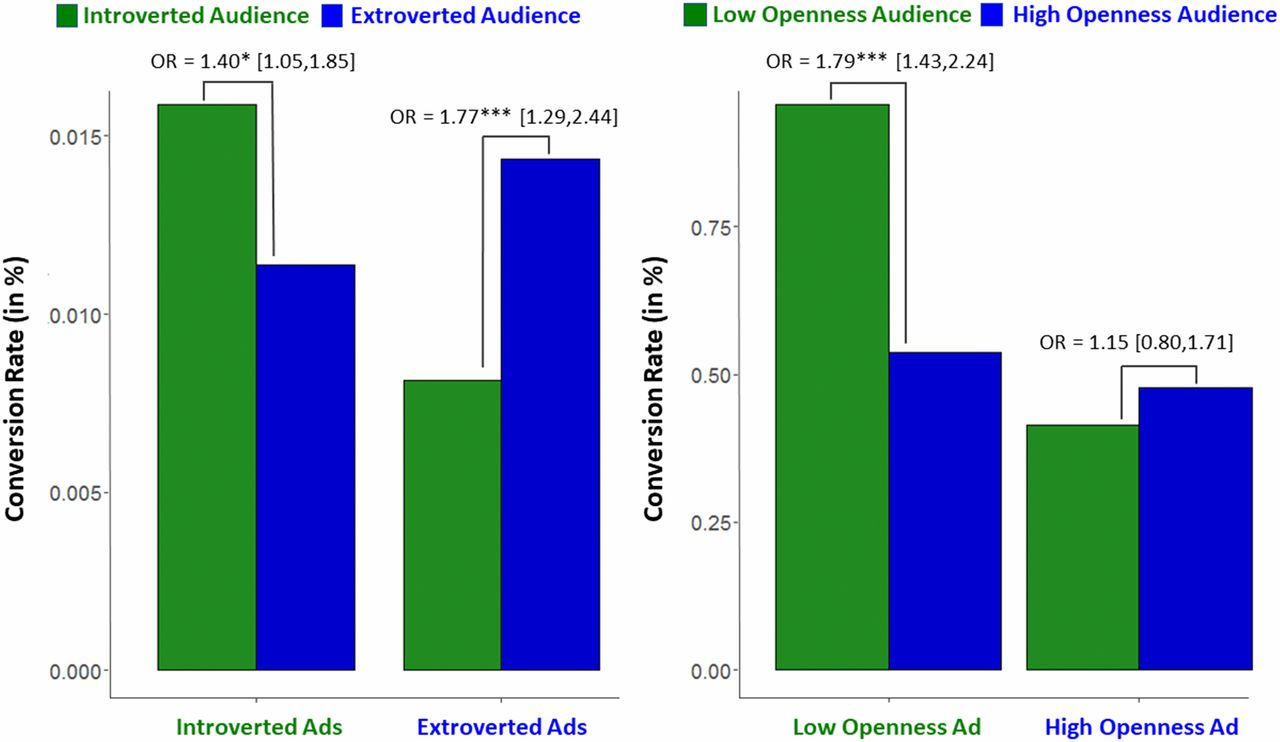
\includegraphics[scale = .8]{png/Kosinski2_S2.jpg}
            \caption{\cite{Matz12714}}
        \end{figure}
    }

\end{frame}


\begin{frame}
    \frametitle{Micro-Targeting in Politics}
    \begin{itemize}
        \item George W. Bush 2004 reelection campaign
        \item Barack Obama 2008 campaign (\href{https://www.youtube.com/watch?time_continue=7&v=BiQwcFRUg_8}{\textcolor{blue}{YouTube clip}})
        \item Ted Cruz and Donald Trump 2016 campaign
    \end{itemize}
\end{frame}

\section[Cambridge Analytica]{How different was Cambridge Analytica Scandal from Micro-Targeting in Politics?}

\section[Cambridge Analytica]{How different was Cambridge Analytica Scandal from Micro-Targeting in Politics}
\begin{frame}[plain,fragile]{Anatomy of the CA scandal}
\begin{tikzpicture}[node distance=1.5cm]
% Specification of nodes (position, etc.)
\node (kogan)   [base] {A. Kogan\\Cambridge Psych.};
\node (life)    [app, below of=kogan] {This is Your Digital Life \\ (FB app)};
\node (user1)   [data, below of=life] {27k users};
\node (user2)   [data, below of=user1] {Indirect access to 87 mln FB profiles};
\node (sold)    [action, right of=life, xshift=1.5cm, yshift=-.5cm] {Sold to};
\node (ca)      [base, right of=sold, xshift=.5cm] {Cambdridge\\Analytica};
\node (other)   [app, below of=ca, yshift=-1cm] {Other data sources\\(e.g. Cruz Crew)};
\node (pc)      [plain, right of=ca, xshift=.5cm] {$\vdots$};
\node (p1)      [data, above of=pc] {Segment $1$};
\node (pn)      [data, below of=pc] {Segment $n$};
\node (micro)   [action, right of=pc, xshift=.5cm] {Microtargeting};
\node (note)    [note, above of=sold, xshift=1cm, yshift=1cm] {Violation of FB policy;\\greyzone in terms of law};
% Specification of paths
\draw[->] (kogan) -- (life);
\draw[->] (life) -- (user1);
\draw[->] (user1) -- (user2);
\draw[->] (kogan) -- (sold);
\draw[->] (user2) -- (sold);
\draw[->] (sold) -- (ca);
\draw[->] (other) -- (ca);
\draw[->] (ca) -- (p1);
\draw[->] (ca) -- (pn);
\draw[->] (p1) -- (micro);
\draw[->] (pn) -- (micro);
\draw[-] (sold) -- (note);
\end{tikzpicture}
\end{frame}


\section[Discussion]{Discussion}
\begin{frame}
    \frametitle{Discussion}
    \begin{enumerate}
        \item Social benefits and risks of using digital footprints.
        \item Social Science benefits and risks of using digital footprints.
    \end{enumerate}
\end{frame}


%%% LITERATURE %%%%%%%%%%%%%%%%%%%%%%%%%%%%%%%%%%%%%%%%%%%%%%%%%%%%%%%%%%%%%%%%
\begin{frame}{Literature}
    \nocite{*}
    \AtNextBibliography{\footnotesize}
    \printbibliography
\end{frame}
